\chapterimage{chapter_head_1.png}

\chapter{Suchalgorithmen für Spiele}

\usetikzlibrary{calc}
\usetikzlibrary{positioning}
\usetikzlibrary{matrix}

\pgfdeclarelayer{background}
\pgfsetlayers{background,main}


\section{Intro \& Motivation}

In den vorangegangenen Kapiteln haben wir schon einige Suchverfahren kennengelernt, welche uns nun helfen werden Algorithmen zu verstehen, die verwendet werden um Computergegner für Nullsummenspiele zu entwickeln. Hierbei werden wir uns den Minimax-Algorithmus, sowie den Alpha-Beta-Algorithmus genauer anschauen, welche beide versuchen sich in die Lage des Gegners zu versetzen, um so  herauszufinden, welche Reaktion dieser auf einen Zug von uns wählen würde. Ziel der Algorithmen ist es, ein für uns best mögliches Ergebnis und somit, wenn möglich, einen Sieg zu erlangen. Dieses Vorgehen kann eine Betrachtung von sehr vielen möglichen Züge zur Folge haben, was sehr viel Rechenaufwand bedeutet. Im Folgenden werden wir jedoch  mit Hilfe des Alpha-Beta-Algorithmus eine Methode kennenlernen, die es uns ermöglicht die Anzahl der zu betrachtenden Züge zu reduzieren.



\section{Inhaltliche Ausarbeitung des Themas}

Wir betrachten ein Nullsummenspiel, was bedeutet, dass der Gewinn des einen Spielers (Nutzwert positiv) mit dem Verlust des Gegners (Nutzwert negativ) äquivalent ist und ein Unentschieden keine Auswirkungen auf die Nullsummeneigenschaft hat (Nutzwert 0).
Gegeben sei für dieses Spiel ein Spielbaum $T = (V;E)$. Bei einem gleichförmigen Spielbaum besitzt jeder innerer Knoten den gleichen Verzweigungsgrad b und alle Blätter befinden sich in der gleichen Tiefe d, , sodass die Zahl der Knoten in einem gleichförmigen Baum exponentiell mit der Tiefe des Baumes wächst ($b^d$). Jedoch gibt es auch Spielbäume bei denen der Verzweigungsgrad der Ebenen variiert.
Der Spielbaum beinhaltet alle möglichen Züge und Spielausgänge. Die Tiefe und der Verzweigungsgrad hängt von dem Spiel ab, welches wir betrachten. Beispielsweise hat der Spielbaum zu einem Tic-Tac-Toe Spiel eine Tiefe von 9 (da es 9 Felder zu besetzen gibt) und zu Beginn des Spiels einen Verzweigungsgrad von 9 (weil noch alle 9 Felder zur Auswahl stehen), der mit wachsender Tiefe allerdings abnimmt, da nach jedem Zug immer ein leeres Feld weniger vorhanden ist.



\subsection{Problemstellung}
Zu dem gegeben Nullsummenspiel wollen wir einen Computergegner programmieren, der in der Lage ist die optimale Antwort auf jede Spielposition, bei optimalem Spiel beider Spieler, zu finden.
Dafür müssen wir jedoch vorher festlegen, was für uns optimal in diesem Zusammenhang bedeutet. Wir gehen davon aus, dass der Gegner immer den für ihn optimalen Zug wählt, dh der Zug, der für ihn zum besten Nutzwert und somit für uns zum schlechtesten Nutzwert führt. Analog wollen wir agieren. Wie dies genau funktioniert werden wir im folgenden Abschnitt sehen.



\subsection{Methoden}


\subsubsection*{Minimax Algorithmus}
Im folgenden bezeichnen wir unseren Spieler mit MAX und den gegnerischen Spieler mit MIN. Wie zuvor schon angedeutet ist das Ziel des Minimax Algorithmus den Minimax-Wert für die aktuelle Stellung zu bestimmen. Der Minimax-Wert der Endstellungen (Blätter) entspricht dem Nutzwert für MAX. Die Berechnung der anderen Knoten erfolgt rekursiv mit Hilfe der folgenden Bewertungsfunktion:

\begin{center}
	$Minimax(k) = \begin{cases} Nutzwert(k) &		,falls~ k ~Endzustand\\
		max\{minimax(t) ~|~ t \in N(t)\} 	&		,falls~ k~ MAX-Knoten\\
		min\{minimax(t) ~|~ t \in N(t)\},	&		,falls~ k~ MIN-Knoten	\end{cases} $
\end{center}

wobei $N(t)$ die Funktion ist, die die Kinder im Baum liefert. Die Auswertung der Knoten geschieht Bottom up, das bedeutet wir beginnen bei den Blättern und bewerten von dort ausgehend die Elternknoten und anschließend deren Eltern bis wir irgendwann bei der Wurzel angelangt sind. Der Minimax Algorithmus liefert nicht unbedingt den höchsten Nutzwert der Blätter, sondern den größten Nutzwert den man erhalten kann, wenn der Gegner selbst versucht zu gewinnen und somit den Nutzwert für uns möglichst klein zu halten.\\

Anschaulicher wird das ganze, wenn man sich den Algorithmus an einem Beispiel anschaut.
\\

\newpage


\textbf{Beispiel}\\

Gegeben sei der folgende Spielbaum
\begin{center}
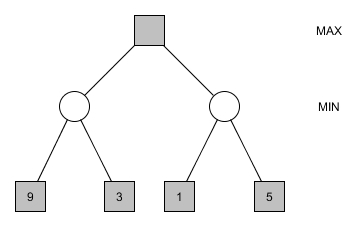
\includegraphics[width = 7 cm]{chapters/minimax/jpg/Graph-Minmax1.jpg}
\end{center}

Angenommen MIN wäre an der markierten Position:
\begin{center}
	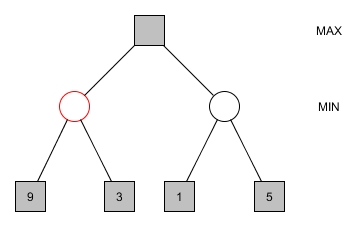
\includegraphics[width = 7 cm]{chapters/minimax/jpg/Graph-Minmax2-1.jpg}
\end{center}

Dann würde MIN den Zug auswählen, der für ihn den größten Nutzwert und somit für uns den kleinsten Nutzwert hat. Das heißt in dem Fall:
\begin{center}
	 $min\{minimax(t) | t \in N(t)\} ~=~ min\{9,3\} ~=~ 3$

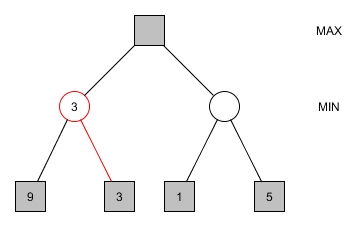
\includegraphics[width = 7 cm]{chapters/minimax/jpg/Graph-Minmax2-2.jpg}
\end{center}

\newpage

Angenommen MIN wäre an der markierten Position:
\begin{center}
	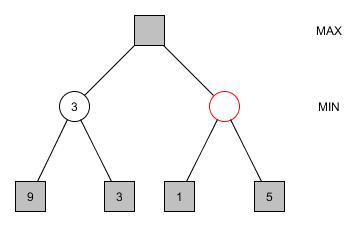
\includegraphics[width = 7 cm]{chapters/minimax/jpg/Graph-Minmax2-3.jpg}
\end{center}

Dann würde MIN den Zug auswählen, der für ihn den größten Nutzwert und somit für uns den kleinsten Nutzwert hat. Das heißt in dem Fall:
\begin{center}
	$min\{minimax(t) | t \in N(t)\} ~=~ min\{1,5\} ~=~ 1$

	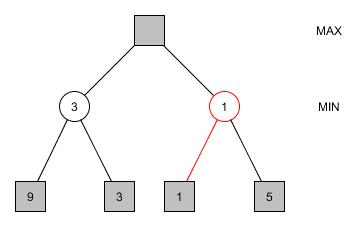
\includegraphics[width = 7 cm]{chapters/minimax/jpg/Graph-Minmax2-4.jpg}
\end{center}

Nun betrachten wir den Zug von MAX. Der Suchbaum sieht wie folgt aus

\begin{center}
	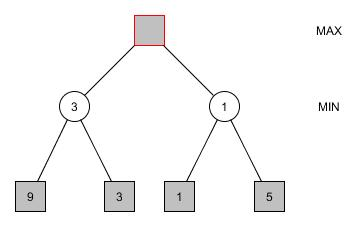
\includegraphics[width = 7 cm]{chapters/minimax/jpg/Graph-Minmax2.jpg}
\end{center}

MAX würde den Zug wählen, der für ihn den höchsten Nutzwert hat.\\

\begin{center}
	$max\{minimax(t) | t \in N(t)\} ~=~ max\{3,1\} ~=~ 3$
	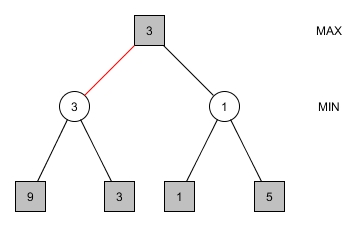
\includegraphics[width = 7 cm]{chapters/minimax/jpg/Graph-Minmax3.jpg}
\end{center}

Somit sieht der Suchbaum nach Abschluss des Minimax-Algorithmus wie folgt aus, wobei der rote Pfad den optimalsten Nutzwert liefert, wenn beide Spieler optimal spielen. Somit sollte MAX den linken Knoten wählen.

\begin{center}
	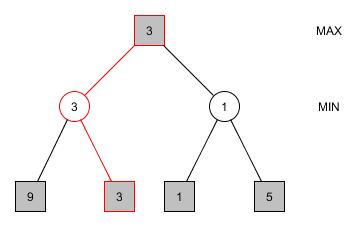
\includegraphics[width = 7 cm]{chapters/minimax/jpg/Graph-Minmax4.jpg}
\end{center}

\vskip 60pt



\subsubsection*{Problem:} Der Minimax-Algorithmus durchsucht den Suchbaum $T=(V, E)$ mit Tiefensuche, in der Zeit $O(max {|V|, |E|}) = O(|V|)$. Somit benötigt die Suche zwar lineare Zeit, jedoch wächst der Baum exponentiell mit zunehmender Tiefe ($O(|V|)=O(b^d)$). Somit ist der Algorithmus für Bäume mit großer Tiefe ineffizient.


\newpage

\subsubsection*{Alpha-Beta-Algorithmus}
 Der Alpha-Beta-Algorithmus ist eine Verbesserung vom Minimax-Algorithmus, da die Zugriffsanzahl reduziert wird, indem Teile des Suchbaums nicht durchsucht werden, ohne dabei das Ergebnis zu verfälschen. Für die Umsetzung werden die Variablen $\alpha$ und $\beta$ eingeführt, wobei $\alpha$ der Nutzwert ist, welchen MAX mindestens erreicht und $\beta$ der Nutzwert, den MIN höchstens erreicht. Die Auswertung der Knoten geschieht on-the-fly, dh nur dann wenn wir sie wirklich benötigen. \\

 \underline{MAX-Knoten:}\\
 Betrachten wir einen MAX Knoten und stellen dort einen Wert fest der größer ist als $\beta$ brauchen wir den Teilbaum nicht weiter betrachten, da MIN diesen nicht wählen würde, weil der andere Teilbaum einen kleineren Nutzwert liefert. Das nicht weiter Betrachten des Teilbaums bezeichnet man als Beta-Cutoff. Ist  der Wert des MAX Knoten größer als $\alpha$ erhöht sich der Wert den MAX mindestens erreicht und wir aktualisieren $\alpha$ auf den Wert des Knotens.  \\

 \underline{MIN-Knoten:}\\
 Ist der Wert eines MIN Knotens kleiner als der Wert von $\alpha$ müssen wir diesen Teilbaum nicht weiter analysieren, da MAX immer den Teilbaum mit dem größten Nutzwert auswählt und da $\alpha$ größer ist als der Wert des betrachteten Knotens existiert ein Teilbaum mit einem größeren Nutzwert. Also würde hier ein Cutoff stattfinden, welchen man als Alpha-Cutoff bezeichnet. Sollte jedoch der Wert des MIN Knotens größer als $\beta$ sein steigt der Wert den MIN höchstens erreicht und wir müssen $\beta$ auf diesen Wert anpassen.


 \begin{algorithm}
 	\KwData{Graph $G=(V,E)$, Blätter mit Nutzwert, s = Knoten}
 	\KwResult{Nutzwert für jeden knoten}
 	\textbf{alpha-beta-suche(s)}\\

 	\textbf{return} maximalerWert(s, -$\infty$, $\infty$)\\

 	\textbf{maximalerWert}(Knoten, $\alpha$, $\beta$)\\

	 	\If{s = Blatt}{
	 		\textbf{return} wert(s)
	 	}
	 	\Else{
	 		$wert = \alpha$\\
	 		\lForEach{k= Kind(s)}{
		 		$wert = max\{wert, minimalerWert(k, wert, \beta)\}$\\
		 		\If {$wert >= \beta$}{
			 		\textbf{return} wert}
			 	$\alpha = max\{\alpha, wert\}$\\
	 		\textbf{return} wert
	 		}
	 	}

	\textbf{minimalerWert}(Knoten, $\alpha$, $\beta$)\\

	\If{s = Blatt}{
		\textbf{return} wert(s)
	}
	\Else{
		$wert = \beta$\\
		\lForEach{k= Kind(Knoten)}{
			$wert = min\{wert, minimalerWert(k, \alpha, wert)\}$\\
			\If {$wert <= \alpha$}{
				\textbf{return} wert}
			$\beta = min\{\beta, wert\}$\\
			\textbf{return} wert
		}
	}
 	\caption{Alhpa-Beta-Algorithmus}
\end{algorithm}
\newpage


Betrachten wir ein Beispiel, um den Algorithmus besser zu verstehen.
\newline

\textbf{Beispiel:}\\

Gegeben sei der folgende Spielbaum:
\begin{center}
	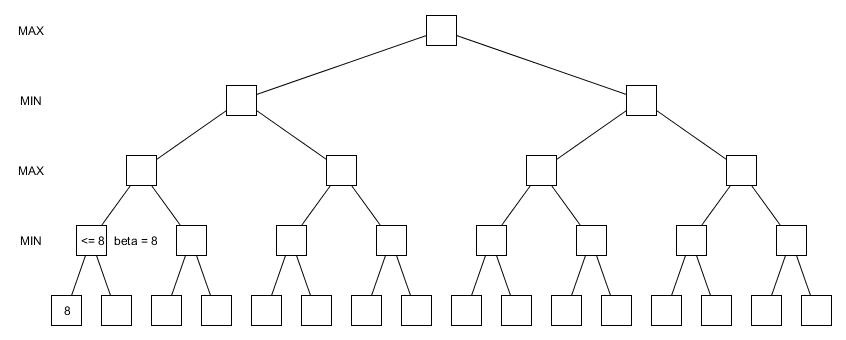
\includegraphics[width = 12 cm]{chapters/minimax/jpg/Alpha-beta1.jpg}
\end{center}

Wir betrachten das erste Blatt. Da MIN immer den Zug mit dem niedrigsten Nutzwert auswählt erreicht er einen Nutzwert $<=8$. Somit ist $\beta = 8$. Da $\beta > \alpha = -\infty$ müssen wir noch das andere Blatt betrachten.

\begin{center}
	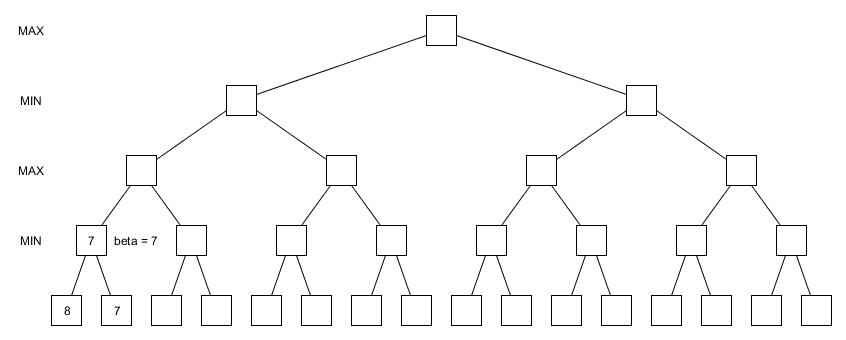
\includegraphics[width = 12 cm]{chapters/minimax/jpg/Alpha-beta2.jpg}
\end{center}

Das zweite Blatt hat den Nutzwert 7, somit ist er kleiner als der aktuelle Wert von $\beta$. Aus diesem Grund erhält der MIN-Knoten den Wert $min\{8,~7\} =7$. Somit ergibt sich für den darüberliegenden Knoten, dass er einen Wert $>=7$ hat, da MAX immer den Knoten mit dem größten Nutzwert auswählt. Nun betrachten wir das Blatt mit dem Nutzwert 3.

\begin{center}
	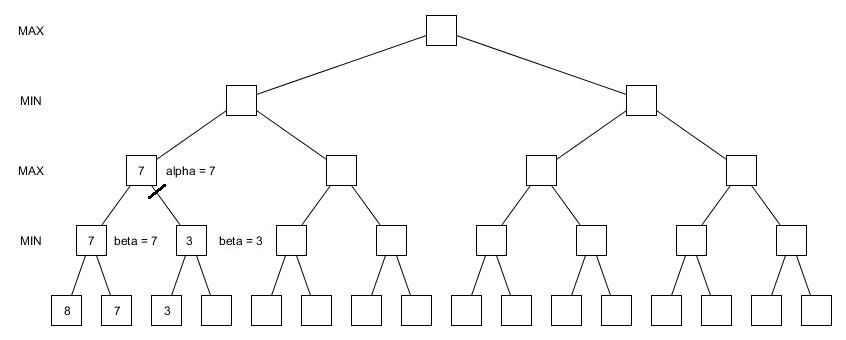
\includegraphics[width = 12 cm]{chapters/minimax/jpg/Alpha-beta3.jpg}
\end{center}

Sein Elternknoten hat für $\alpha$ den Wert 7 (MAX erreicht mind. eine 7) und $\beta$ hat den Wert 3 (MIN erreicht höchstens den Wert 3). Vergleicht man $\alpha$ und den Wert des MIN Knotens fällt auf, dass $\alpha$ > 3 was bedeutet, dass man den Teilraum nicht weiter betrachten muss und hier ein Cutoff durchgeführt wird. Anders ausgedrückt MAX würde nicht diesen Zug wähle, da der andere Zug einen Nutzwert von 7 liefert und dieser nur einen von maximal 3.

\begin{center}
	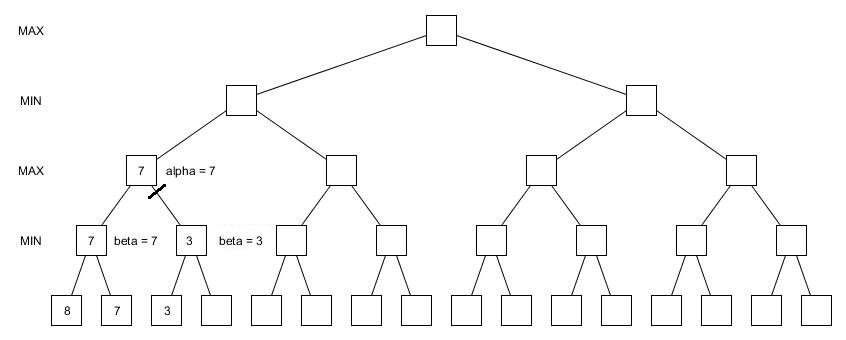
\includegraphics[width = 12 cm]{chapters/minimax/jpg/Alpha-beta3-1.jpg}
\end{center}

Somit erreicht MAX an dem Knoten einen Nutzwert von 7 und der darüber liegende MIN Knoten einen Wert von $<=7$, was bedeutet, dass $\beta = 7$. Betrachten wir nun das nächste Blatt, welches den Nutzwert 9 hat.

\begin{center}
	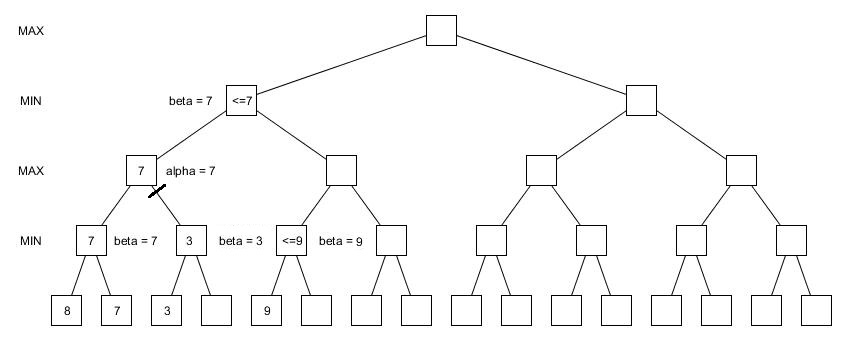
\includegraphics[width = 12 cm]{chapters/minimax/jpg/Alpha-beta4.jpg}
\end{center}

 Da $-\infty = \alpha <9$ müssen wir auch das nächste Blatt betrachten. Anders ausgedrückt, wir können nicht ausschließen das MIN das rechte Blatt wählen würde.

 \begin{center}
 	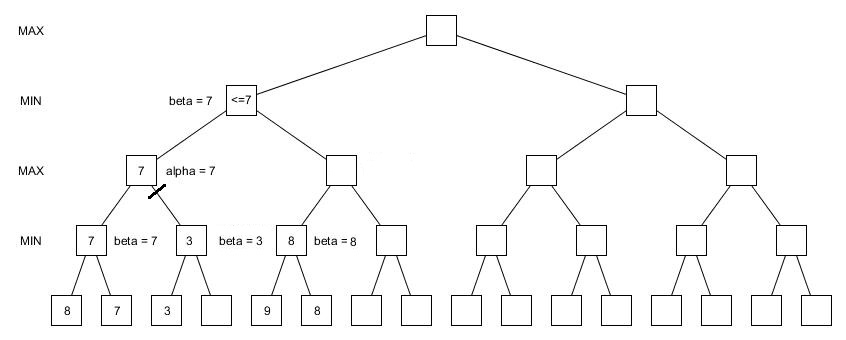
\includegraphics[width = 12 cm]{chapters/minimax/jpg/Alpha-beta5.jpg}
 \end{center}

 Da das nächste Blatt den Nutzwert 8 hat, würde MIN diesen Zug wählen, da sein Nutzwert kleiner ist als der des anderen Zuges ($min\{\beta, 8\}= min\{9,8\}=8$). Somit aktualisiert sich der Wert von $\beta$ auf 8.

 \begin{center}
 	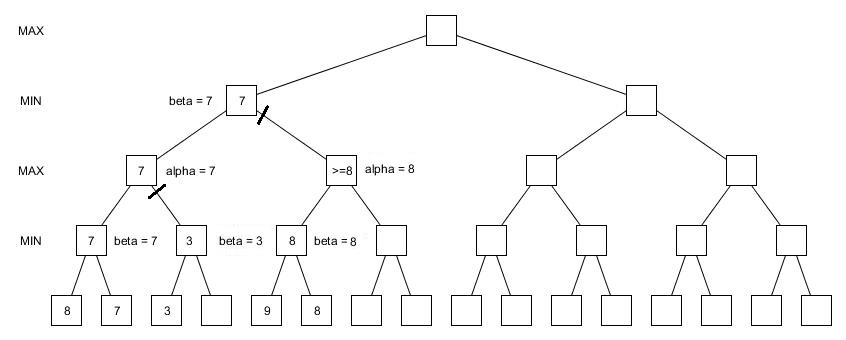
\includegraphics[width = 12 cm]{chapters/minimax/jpg/Alpha-beta6.jpg}
 \end{center}

 Dies hat zur Folge das $\alpha =8$, da MAX im darüber liegenden Zug mindestens einen Nutzwert von 8 erreicht. Somit hat er einen größeren Wert als der linke MAX Knoten, weshalb sich MIN nicht den rechten Knoten aussuchen würde und wir somit auch den Teilbaum nicht weiter betrachten müssen. Anders ausgedrückt, da für den rechten Teilbaum der MAX Knoten einen Wert von mindestens 8 hat und  $\beta = 7$ ist, gilt $\beta<8$ und es findet ein Cutoff statt.  Aufgrund dessen hat der MIN Knoten den Wert 7.

 \begin{center}
 	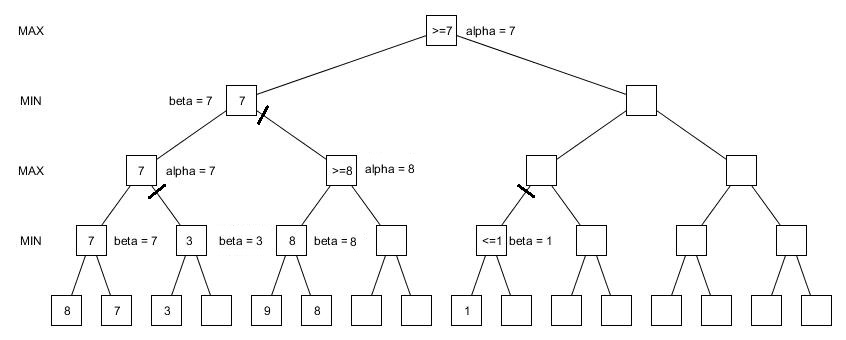
\includegraphics[width = 12 cm]{chapters/minimax/jpg/Alpha-beta7.jpg}
 \end{center}

 Für die Wurzel ergibt sich somit ein Wert von mindestens 7 und $\alpha = 7$
 Die Betrachtung des nächsten Blattes liefert das der MIN Knoten höchstes den Wert 1 hat. Da 1 <$\alpha$ ist eine weitere Betrachtung des Teilbaumes nicht nötig und wir können ihn abschneiden. Mit anderen Worten würde MAX nicht den Zug dieses Teilbaumes wählen, da der Nutzwert des linken Teilbaumes einen höheren Nutzwert hat.

 \begin{center}
 	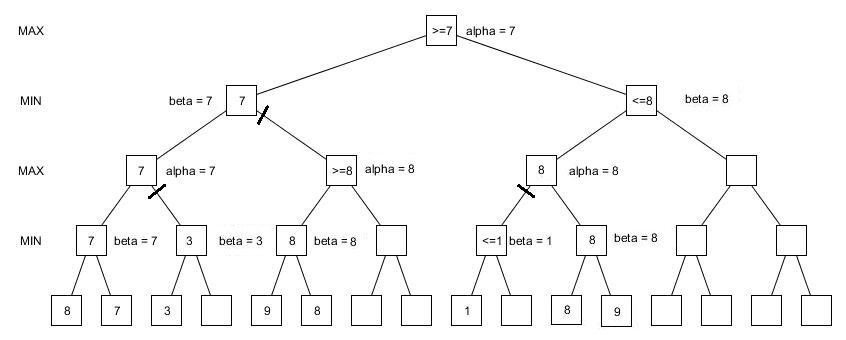
\includegraphics[width = 12 cm]{chapters/minimax/jpg/Alpha-beta8.jpg}
 \end{center}

 Die Auswertung der nächsten beiden Blätter und ihres Elternknotens liefert keine Cutoffs.

 \begin{center}
 	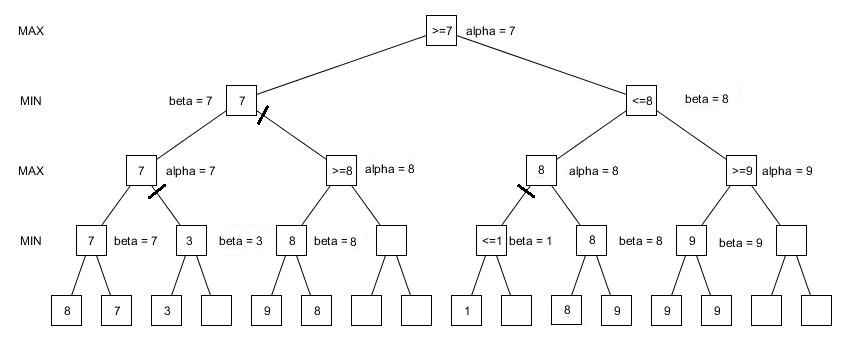
\includegraphics[width = 12 cm]{chapters/minimax/jpg/Alpha-beta9.jpg}
 \end{center}

 Betrachtet man nun die nächsten beiden Blätter liefert das einen Nutzwert von 9 für den MIN Knoten ($\beta =9$) und somit für den MAX Knoten einen Wert $>=9$. Der darüber liegende MIN Knoten würde jedoch nicht den rechten Knoten mit einem Nutzwert $>=9$ wählen, da der linke Knoten nur einen Nutzwert von 8 hat. Somit ist eine weitere Betrachtung des Teilbaumes nicht nötig.\\
 Dies ist somit der endgültige Spielbaum.

 \begin{center}
 	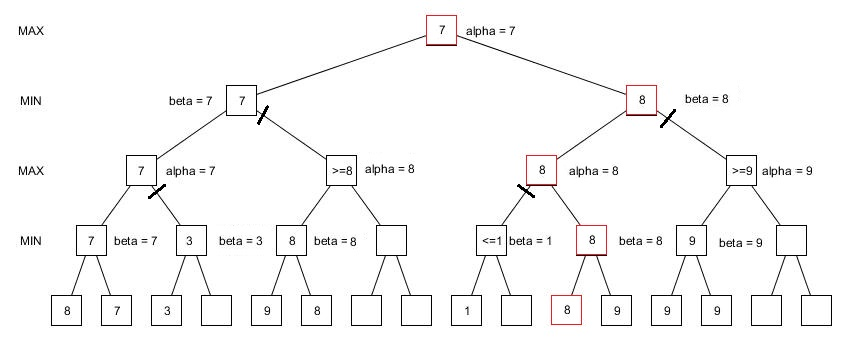
\includegraphics[width = 12 cm]{chapters/minimax/jpg/Alpha-beta10.jpg}
 \end{center}

 Der rot gekennzeichnete Pfad ist der Pfad, der den höchsten Nutzwert liefert, wenn beide Spieler, so wie von uns zu Beginn angenommen, optimal Spielen. Dies bedeutet für den ersten Zug von MAX , das er den rechten Knoten wählen sollte.
 \newline

 Für die Berechnung dieses Pfades mussten wir uns 23 Knoten anschauen, wohingegen wir beim Minimax-Algorithmus alle 31 Knoten hätten betrachten müssen, um zu diesem Ergebnis zu gelangen. Somit bietet der Alpha-Beta-Algorithmus in diesem Beispiel eine deutliche Rechenzeitverbesserung.



\section{Abgrenzung / Vergleich zu den vorherigen Kapitel}

In den vorherigen Kapiteln haben wir verschiedene Suchalgorithmen (Bestensuche, Branch-and-Bound, A*) kennengelernt. Diese liefern den Pfad, der zu dem Blatt mit dem höchsten Nutzwert führt. Jedoch beachten sie nicht, ob der Gegner auch diesen Pfad wählen würde. Der Gegner würde versuchen den geringsten Nutzwert für uns zu erreichen und somit versuchen von diesem Pfad abzuweichen.Folglich würden sie keine realistische Einschätzung darüber geben, welche Züge das beste Spielergebnis liefern. Im Gegensatz dazu betrachten sowohl der Minimax, als auch der Alpha-Beta Algorithmus das Verhalten des Gegners, welches zu einer guten Einschätzung der Spielsituation führt.



\section{Fazit \& Bewertung}

Zusammenfassend lässt sich sagen, dass der Minimax- und der Alpha-Beta-Algorithmus zum selben besten Ergebnis für den MAX Spieler führen und sich lediglich in ihrer Effizienz unterscheiden können, da der Alpha-Beta-Algorithmus weniger Berechnungen und somit eine kürzere Rechnungszeit benötigen kann. Je nach Suchbaum kann die Anzahl der Cutoffs und die Einsparung der Rechenzeit sehr groß ausfallen. Aufgrund dessen ist der Alpa-Beta-Algorithmus eine Grundlage für viele Algorithmen im Bereich der Nullsummenspiele für zwei Personen. Für die Berechnungen der Algorithmen sind die Werte der Blätter von größer Bedeutung, welche durch die Heuristik gegeben sind. Alles in allem kann man sagen, dass man sowohl mit Minimax als auch mit Alpha Beta einen Computergegner programmieren kann, der es einem Menschen sehr schwer, wenn nicht sogar unmöglich, macht zu gewinnen und somit eine künstliche Intelligenz bei Nullsummenspielen für die Zukunft denkbar ist.



\section{Quellen und Literatur}

MIT - Lecture 6: Search: Games, Minimax, and Alpha-Beta\\
http://home.in.tum.de/~adorf/pub/alphabeta-seminar-paper.pdf\\
https://de.wikipedia.org/wiki/Minimax-Algorithmus\\
https://de.wikipedia.org/wiki/Alpha-Beta-Suche

\end{document}
